\documentclass{beamer}
%Information to be included in the title page:
\title{Le problème des dominos de Wang}
\author{Matteo Wei et Nathan Boyer}
\date{2024}
\graphicspath{ {./images/} }
\AtBeginSection[]

\newcommand{\sube}{\subseteq}

\begin{document}

\frame{\titlepage}

\begin{frame}
    \frametitle{Table of Contents}
    \tableofcontents[]
  \end{frame}
  
\section{Introduction}
\begin{frame}
\frametitle{Ensemble de Wang}

\begin{alertblock}{Definition}

    Un \emph{ensemble de Wang} est un triplet $(H,V,T)$ où $H$ et $V$ sont respectivement les couleurs horizontales et verticales
    et où $T \sube H^2 * V^2$ est l'ensemble des dominos. On appelera parfois aussi abusivement ensemble de Wang l'ensemble des dominos $T$.
    
\end{alertblock}

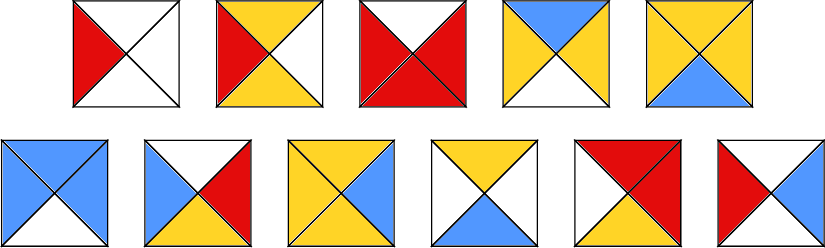
\includegraphics{ensemble_de_wang_exemple}

\end{frame}

\end{document}



